\subsubsection{Submódulo Comunicación inalámbrica}
Por parte de las pruebas de la comunicación inalámbrica se utilizó como apoyo la aplicación móvil Bluetooth Terminal HC-05, con el fin de mostrar los datos enviados por el módulo bluetooth. 
Los datos que serán recibidos serán los pulsos por segundo que el microcontrolador recibe por parte del caudalimetro, es decir la frecuencia de flujo de liquido en cada segundo; estos datos se mostraran en formato hexadecimal.
\\ En la imagen \ref{fig:bt_datos_ceros} se muestran los resultados obtenidos por la aplicación tras no pasar flujo por el caudalimetro, como se puede observar la frecuencia obtenida es cero, lo cual nos muestra un funcionamieto correcto por parte de la transmición de datos del módulo bluetooth y del microcontrolador.
\begin{figure}[H]
	\centering
	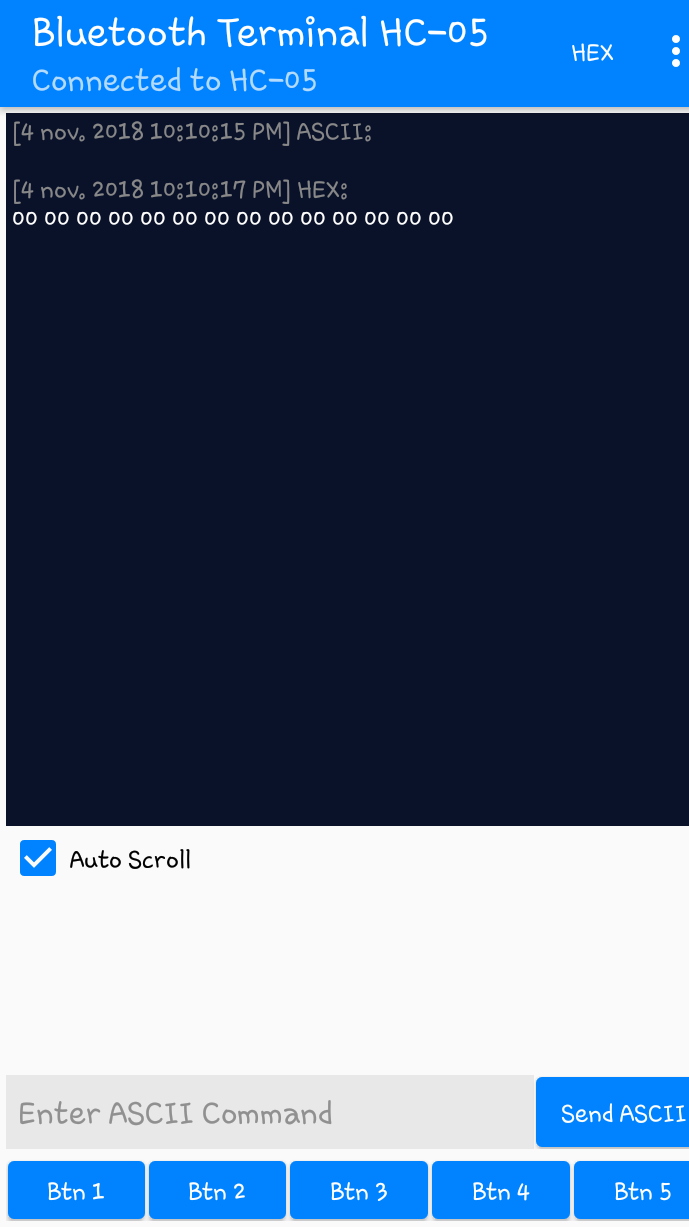
\includegraphics[width=.5\textwidth]{Capitulo6/unitarias/hardware/img/bt_datos_ceros}
	\caption{Datos obtenidos sin recibir flujo en el caudalimetro}
	\label{fig:bt_datos_ceros}
\end{figure}
Para la segunda prueba se introdujeron 300ml de agua por el caudalimetro de manera intermitente, esto con el fin de mostrar los datos enviados por el módulo bluetooth cuando la frecuencia es igual a cero y cuando es distinta de cero. Los resultados se muestran el la figura \ref{fig:bt_datos_flujo}.
\begin{figure}[H]
	\centering
	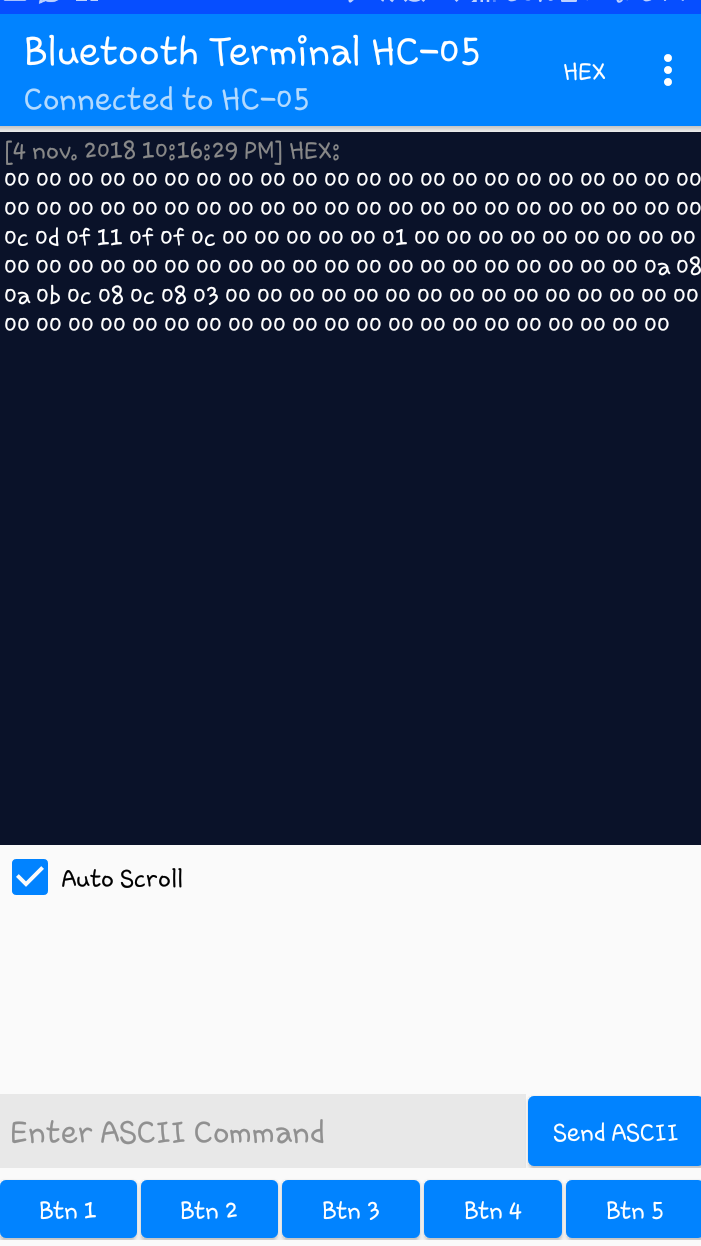
\includegraphics[width=0.5\textwidth]{Capitulo6/unitarias/hardware/img/bt_datos_flujo}
	\caption{Datos obtenidos recibiendo flujo por el caudalimetro}
	\label{fig:bt_datos_flujo}
\end{figure}
Como se pudo visualizar en las pruebas el funcionamiento del microcontrolador y del módulo bluetooth para el envío de los datos de la frecuencia es correcto, estos datos posteriormente se analizaran en la aplicación móvil con el fin de obtener la cantidad de flujo de gasolina que pasa a través del sensor.